\subsection{Julia}
Julia è un linguaggio di programmazione ad alto livello, 
multi-paradigma e open-source ideato per compiere analisi 
numerica ed effettuare operazioni di computer science in 
maniera rapida e stabile. Julia è nato ufficialmente come 
linguaggio di programmazione nell’anno 2012 con lo scopo di 
fornire uno strumento potente, robusto e veloce tanto se non 
più dei linguaggi considerati in questo ambito lo stato 
dell’arte, ovvero C e Fortran;  ma anche facile da approcciare, 
al contrario dei linguaggi sopra citati. Julia è un linguaggio 
di programmazione scritto in C++ e Scheme, ma gran parte della 
sua composizione è scritta in Julia stesso.

le caratteristiche principali di questo linguaggio sono 
principalmente:
\begin{itemize}
    \item Alte performance: lo scopo per cui Julia è nato è 
    stato quello di offrire un linguaggio estremamente 
    performante con la capacità di poter compilare programmi 
    in codice nativo per molteplici piattaforme grazie 
    all’utilizzo di LLVM

    \item Dinamico: la scelta di rendere Julia un linguaggio 
    dinamicamente tipizzato lo rende di facile utilizzo in 
    quanto rende molto più semplice il suo approccio anche a 
    chi non ha una base solida di programmazione, in quanto 
    ritorna la stessa sensazione di immediatezza di un 
    linguaggio di scripting. Inoltre questo permette un alto 
    supporto per l’uso interattivo

    \item Ambiente riproducibile: lo scopo del linguaggio è 
    quello di poter permettere all’utente di ricreare le 
    stesse condizioni ogni volta su ogni macchina su cui un 
    programma viene eseguito. Questo può essere ottenuto 
    tramite l’utilizzo di file binari pre compilati
    \item Componibile: Julia utilizza l’approccio multiple 
    dispatch come paradigma, permettendo una grande 
    flessibilità nell’esprimere una elevata quantità di 
    pattern di programmazione, dall’object-oriented al 
    funzionale
    \item General Purpouse: lo scopo del linguaggio è quello 
    di creare un ecosistema in grado di poter soddisfare 
    qualsiasi esigenza di un utente, permettendo la creazione 
    di applicativi e microservizi senza dover ricorrere ad 
    integrazioni con codice non nativo Julia
    \item Open source: Julia abbraccia la filosofia open source, 
    e il codice sorgente dell’intero linguaggio, così come di 
    tutte le librerie è disponibile sulla piattaforma GitHub 
    sotto la licenza MIT. Questo permette una crescita 
    eterogenea grazie al contributo di più di 1000 utenti 
    che si impegnano a migliorare il linguaggio
\end{itemize}

\subsubsection{Agents.jl}
Seguendo la filosofia propria del linguaggio di programmazione 
in cui è sviluppata, la libreria Agents.jl \cite{Agents.jl} 
viene sviluppata con l’obiettivo di essere facile da imparare e 
usare ed estendibile, con forte attenzione sulla creazione ed 
evoluzione di modelli veloci e soprattutto scalabili. 
Molteplici esempi comparativi sono stati effettuati mostrando 
come il framework sviluppato permetta di avere un notevole 
guadagno prestazionale rispetto ai maggiori competitor 
attualmente presenti sul mercato (Mesa, Netlogo, MASON) 
\cite{ABAR201713}.

\begin{minipage}{\linewidth}
    \centering
    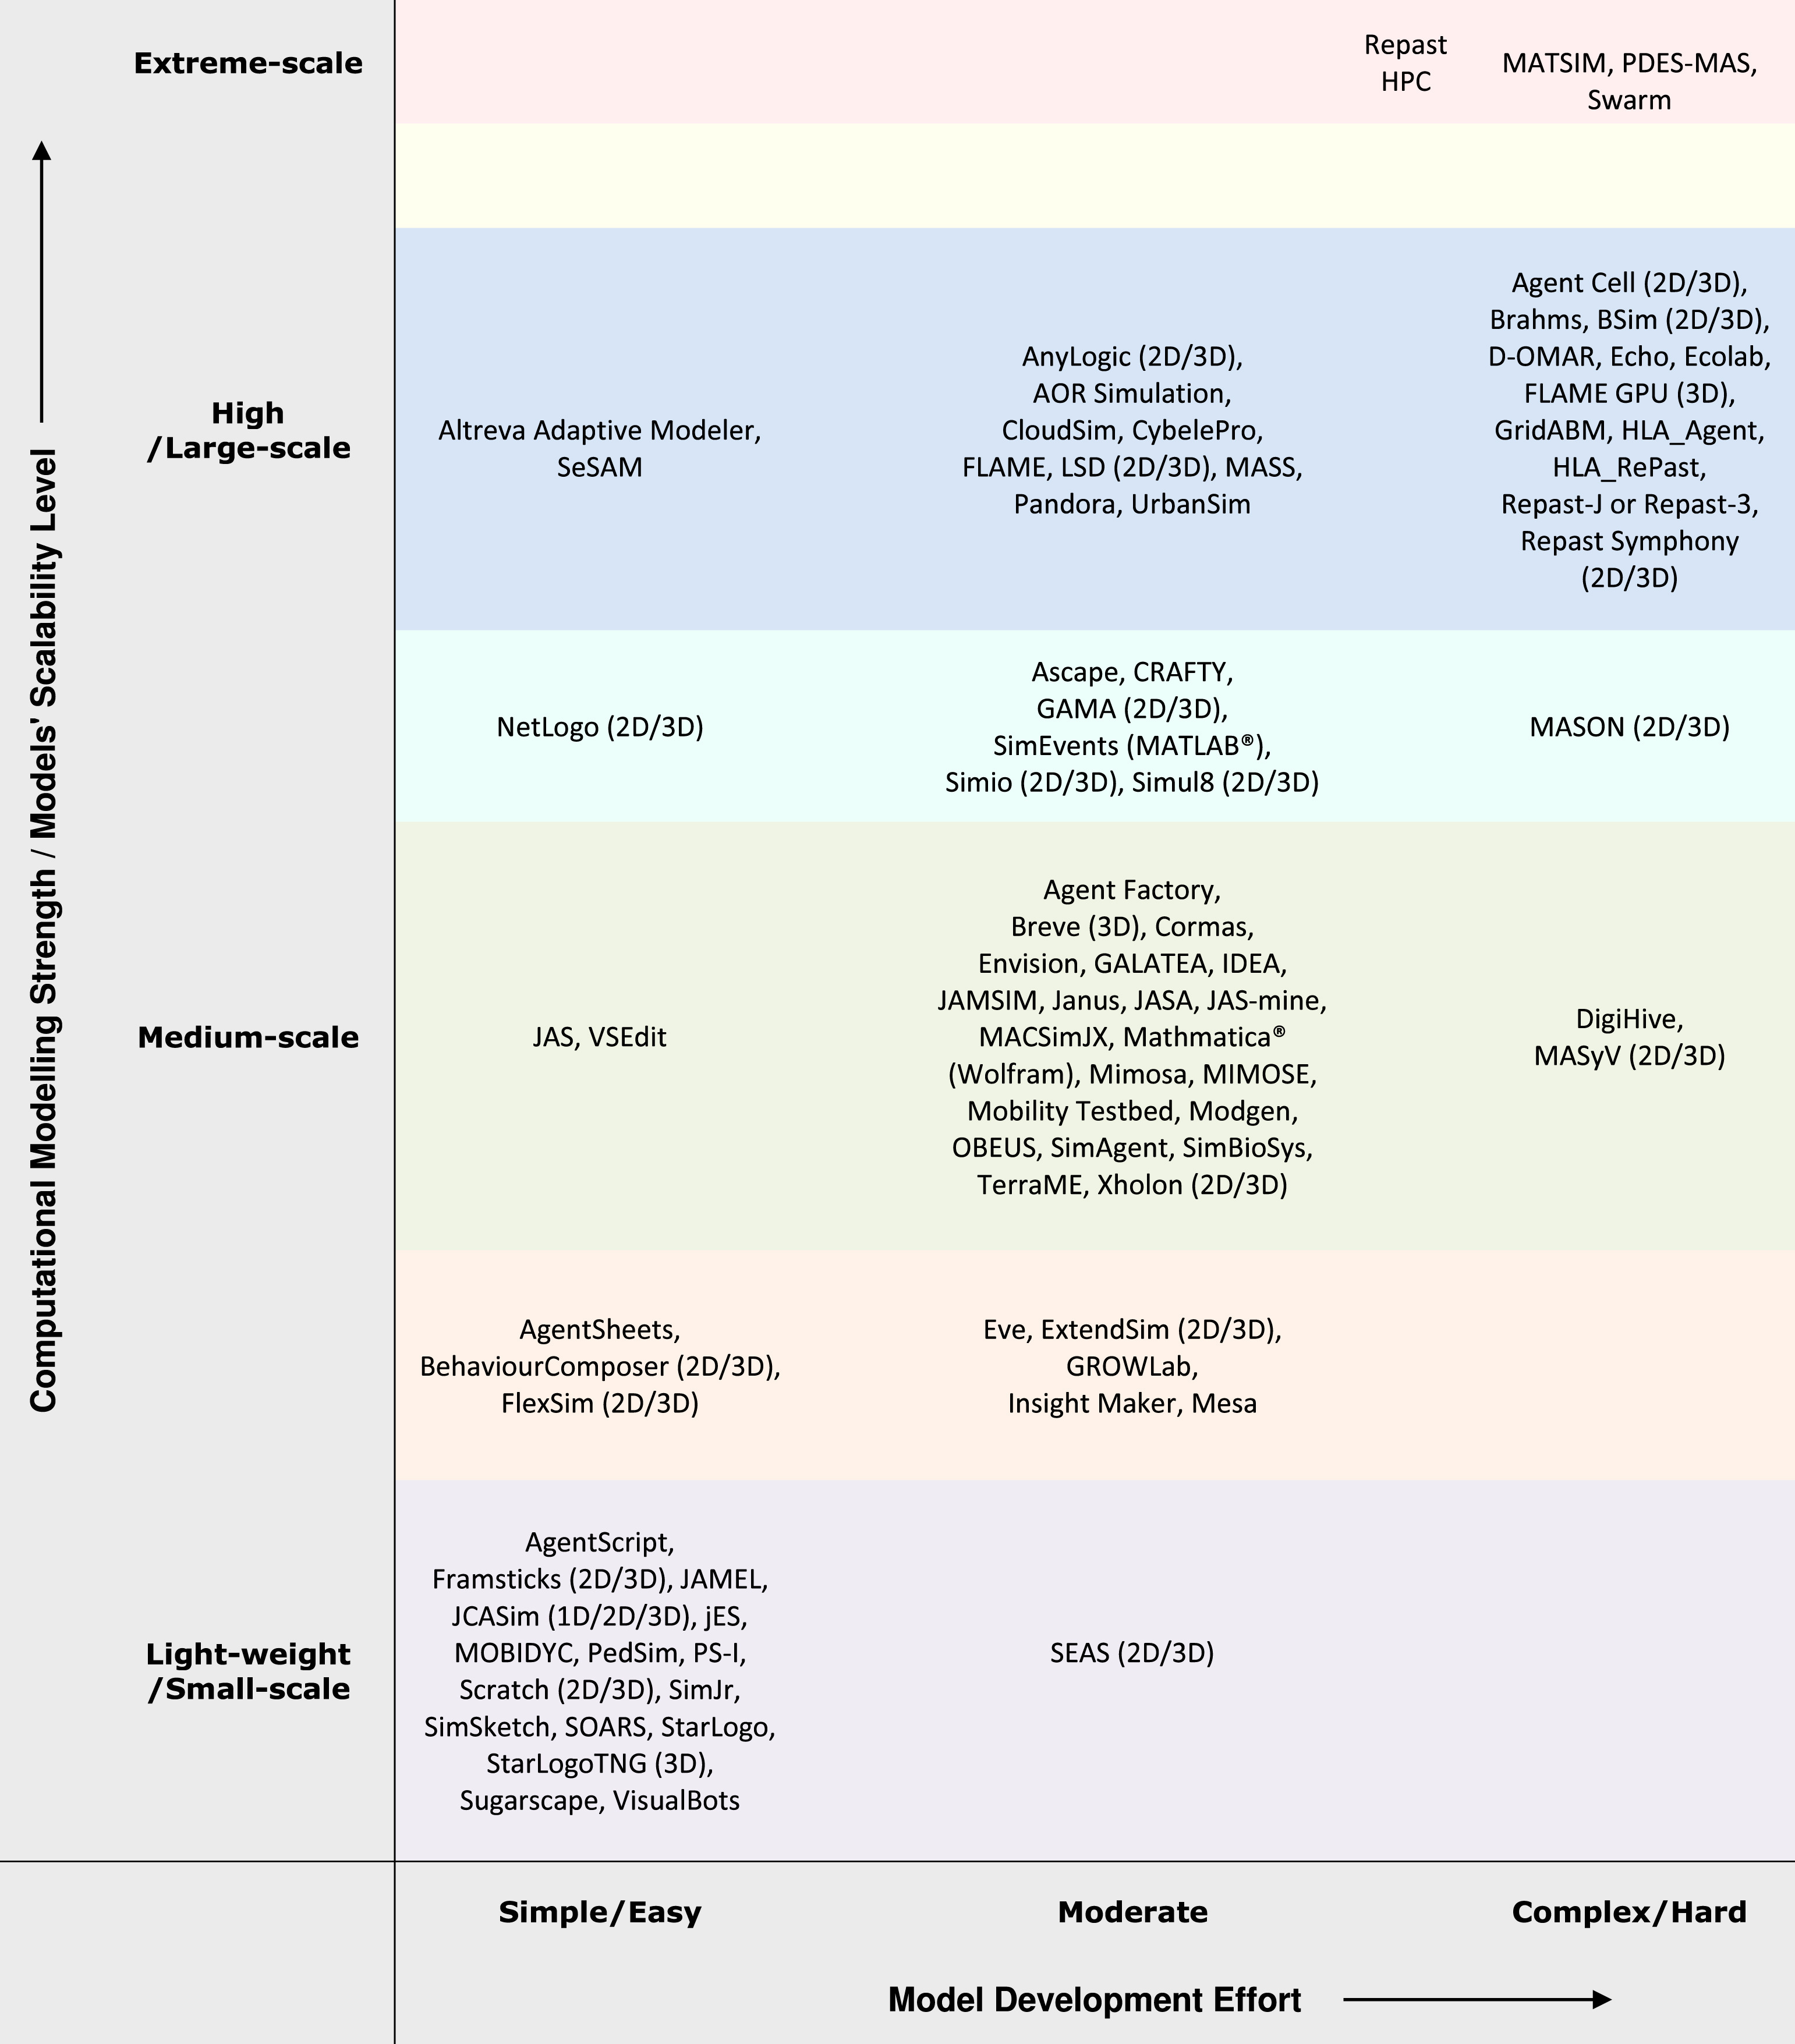
\includegraphics[width=\textwidth]{img/1-s2.0-S1574013716301198-gr1_lrg.jpg}
    \captionof{figure}{Tabella comparativa \cite{ABAR201713}}
    \label{fig:Comparative_table}
\end{minipage}

La facilità di interazione con questa libreria non è da 
confondersi con una mancanza di opzioni durante lo sviluppo, 
in quanto nativamente Agents.jl permette l’integrazione con 
altre librerie che in maniera altrettanto semplice e veloce 
offrono all’utente la possibilità 
di addentrarsi nel mondo del machine learning, in particolar 
modo il mondo del Scientific Machine Learning 
\cite{rackauckas2017differentialequations}, 
branca che soprattutto grazie alla pandemia da Covid-19 ha 
visto un sempre più crescente interesse. 

Agents.jl offre molteplici opzione di configurazione, ma 
principalmente quello su cui si basa sono i seguenti principi:

\begin{itemize}
    \item definizione di un tipo di agente, generalmente viene raccomandato di 
    estendere la tipologia \emph{StandardABM} la quale è la più concreta implementazione,
    nonchè l'implementazione di default, di un costruttore generico di un \textbf{AgentBasedModel}.
    \item definizione di una tipologia di spazio, esistono principalmente 2 tipologie 
    di spazio da poter utilizzare come base e si basano sull'utilizzo di uno spazio \emph{discreto}
    oppure \emph{continuo}.
    \begin{itemize}
        \item spazio discreto a grafo: un \emph{GraphSpace} rappresenta uno spazio del modello
        rappresentato da un grafo arbitrario in cui ogni nodo può contenere una 
        quantità di agenti abitraria. Per funzionare correttamente questa tipologia di 
        spazio richiede che gli agenti implementino al loro interno specifici attributi
        per rappresentare la loro posizione all'interno dello spazio. Questa tipologia di spazio
        si appoggia alla libreria \textbf{Graphs.jl} \cite{Graphs2021} per gestire tutte le operazioni relative
        alla struttura dati del grafo.  

        \begin{minipage}{\linewidth}
            \centering
            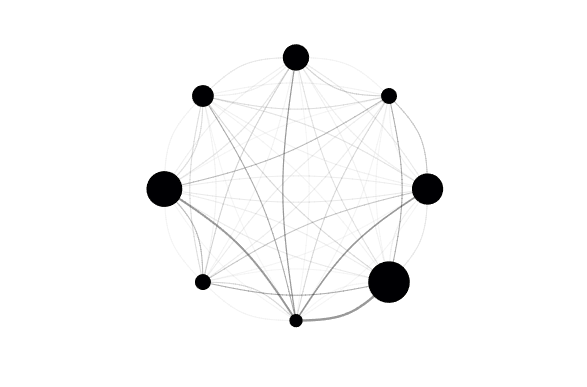
\includegraphics[width=\textwidth]{img/graph.png}
            \captionof{figure}{Esempio di rappresentazione di uno spazio a grafo con archi pesati}
            \label{fig:graphspace_representation}
        \end{minipage}
        
        \item spazio discreto a griglia: un \emph{GridSpace} rappresenta uno spazio del modello
        rappresentato da una griglia di dimensione D $\geq$ 1. Questa tipologia di spazio 
        richiede l'utilizzo di una metrica per la definizione della distanza
        tra celle di una griglia. Ci sono attualmente tre tipologie di metriche supportate 
        e sono: \emph{Euclidean}, \emph{Manhattan} e \emph{Chebyshev}.

        \begin{minipage}{\linewidth}
            \centering
            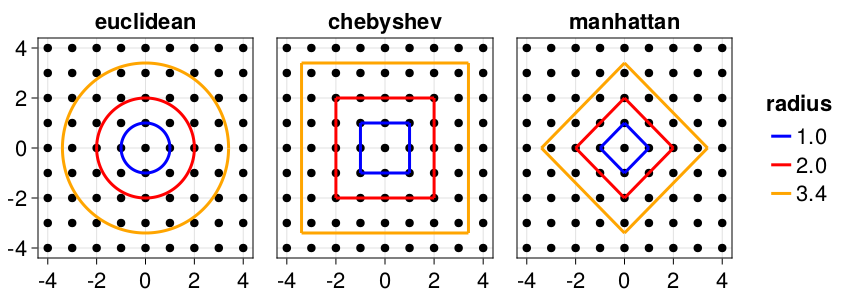
\includegraphics[width=\textwidth]{img/distance.png}
            \captionof{figure}{Esempio di metriche per il calcolo della distanza su uno spazio a griglia}
            \label{fig:gridspace_distances}
        \end{minipage}
        
        \item spazio continuo: un \emph{ContinuousSpace} rappresenta uno spazio di dimensione
        D $\in$ (0, $\infty$). è fortemente consigliato di attribuire ad un agente all'interno 
        di questo spazio due caratteristiche fondamentali, una posizione e una velocità. Questa 
        tipologia di spazio permette di rappresentare delle proprietà spaziali tramite valori 
        finiti oppure tramite \emph{funzioni}, i quali rappresentano una discretizzazione di 
        valori spaziali che potrebbero non essere disponibili in maniera analitica. Utilizzando questa 
        tipologia di spazio la metrica di distanza utilizzata sarà sempre \emph{Euclidian}.
        Per velocizzare il calcolo della posizione degli agenti, viene effettuata una discretizzazione
        implicita dello spazio, ma questa può essere forzata a rimanere nello spazio continuo 
        ottenendo un calo di prestazioni.

        \item spazio misto: un \emph{OpenStreetMapSpace} rappresenta una mappa come un'entità 
        continua che preferisce l'accuratezza alle prestazioni. La mappa viene rappresentata 
        come un grafo connesso. I nodi non rappresentano necessariamente intersezioni. 
    \end{itemize}
\end{itemize} 


\subsubsection{SciML.ai}
SciML.ai è una collezione di librerie dedite all'analisi numerica e 
al calcolo scentifico. Questo framework permette di 
avere tutti gli strumenti per poter utilizzare facilmente, 
velocemente e in maniera robusta tecniche di analisi numerica 
molto avanzata, così da poter sviluppare applicazioni complesse 
in maniera semplice e concreta
\cite{rackauckas2017differentialequations} 
\cite{rackauckas2019diffeqflux} 
\cite{rackauckas2020universal}. 

Il principale utilizzo che è stato fatto di queste librerie si 
concentra principalmente sull'implementazione di metodi di analisi 
numerica, come ad esempio l'utilizzo di di risolutori per sistemi 
di \emph{Equazioni Ordinarie Differenziali} (ODE) che si possono 
trovare nel package \emph{OrdinaryDiffEq.jl} \cite{rackauckas2017differentialequations} 
uniti a metodi di \emph{Machine Learning} (ML) \cite{pal2023lux} \cite{Flux.jl-2018} \cite{innes:2018}
per lo sviluppo di un modello di \emph{Scientific Machine Learning} che si 
appoggia sui costrutti denominati \textbf{Neural Differential Equation (Neural DE)}
e \textbf{Universal Differential Equation (UDE)} 
\cite{rackauckas2019diffeqflux} \cite{rackauckas2020universal}. 

\begin{minipage}{\linewidth}
    \centering
    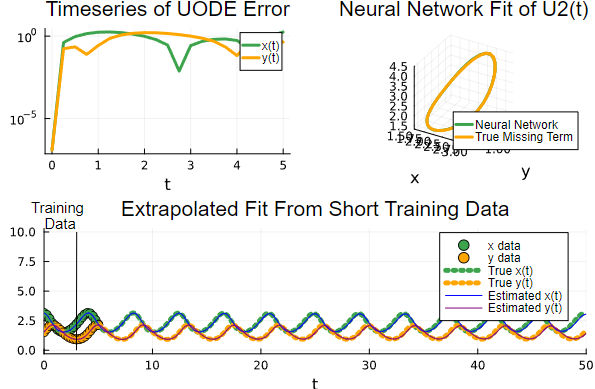
\includegraphics[width=\textwidth]{img/uode_cont.png}
    \captionof{figure}{Esempio applicazione UODE e Neural ODE}
    \label{fig:SciML_example}
\end{minipage}

\subsubsection*{Equazioni Neurali Differenziali}
Da quando l'articolo \cite{chen2019neural} è stato pubblicato questa tecnica
ha ricevuto molta attenzione facendo si che si iniziasse ad ibridare due paradigmi di modellazione come
le ODE e le reti neurali (NN)  per cercare di ottenere il massimo da entrambe minimizzando 
gli effetti indesiderati. \cite{Kim_2021} \cite{chen2019neural}

Un'equazione differenziale è un modo per specificare una trasformazione 
non lineare arbitraria codificando matematicamente le ipotesi strutturali 
a priori del sistema. A riguardo esistono 3 approcci comuni per definire una 
trasformazione non lineare:

\begin{itemize}
    \item \textbf{modellazione diretta}
    \item \textbf{machine learning}
    \item \textbf{equazioni differenziali}
\end{itemize}

Il primo approccio, ovvero la modellazione diretta, funziona solamente se si 
conosce l'esatta funzione che mette in correlazione l'input con l'output. 
Tuttavia nella generalità dei casi questa relazione non è conosciuta a 
priori per cui non è possibile applicare questo approccio. A tal proposito
si può utilizzare l'approccio del machine learning. 

In un generico problema di machine learning dato un insieme di dati $x$ si 
vuole predire un insieme $y$ di dati correlati da una funzione sottostante.
Questa generazione di dati $y$ da $x$ è generalmente definito \emph{modello}. 
L'idea alla base è avere un periodo di allenamento (training) in cui si tenta 
di aggiustare i parametri (iperparametri) del modello così da assicurarsi di 
avere un modello in grado di generare previsioni accurate. Successivamente 
questo modello verrà utilizzato per effettuare inferenza su dati $x$ mai visti. 
Questo approccio è semplicemente un insieme di trasformazioni non lineari. 

\begin{minipage}{\linewidth}
    \centering
    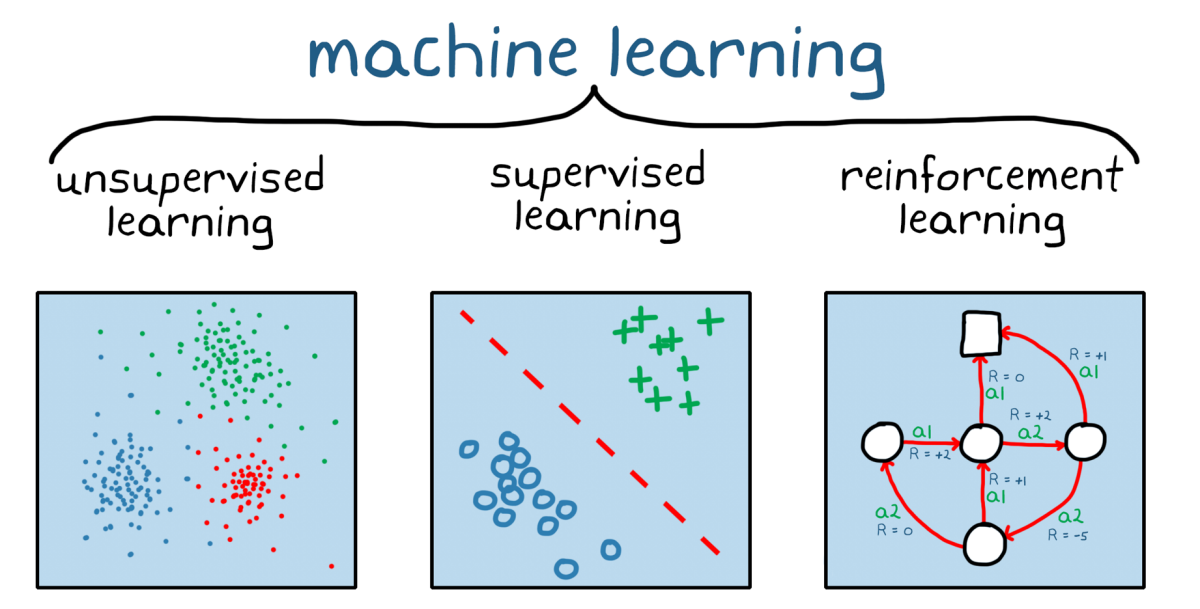
\includegraphics[width=\textwidth]{img/1689243301131.png}
    \captionof{figure}{Differenti approcci di apprendimento di machine learning}
    \label{fig:ML_example}
\end{minipage}

L'utilizzo del machine learning è molto interessante in quanto il concetto 
alla base è estremamente semplice ma è molto potente in quanto riesce ad 
adattarsi ai dati forniti in maniera molto buona. Questa soluzione si espande 
successivamente all'idea di rete neurale (o Neural Network, NN) la quale 
non è altro che un insieme di moltiplicazioni tra matrici seguite
dall'applicazione di una funzione di attivazione. Per esempio una semplice 
rete neurale da 3 strati di profondità viene definita come:

$$ML(x) = \sigma(W_3 \cdot \sigma(W_2 \cdot \sigma(W_1 \cdot x)))$$

dove $W_1$, $W_2$ e $W_3$ sono dei parametri apprendibili. Successivamente 
lo scopo è quello di scegliere $W$ tale che $ML(x) = y$ si comporti in maniera
ragionevole simile alla funzione incognita che vogliamo adattare. Grazie all'
applicazione del teorema di approssimazione universale 
afferma che per un numero sufficientemente grande di parametri o di strati 
è possibile approssimare qualsiasi funzione non lineare in maniera 
sufficientemente precisa. 

\begin{minipage}{\linewidth}
    \centering
    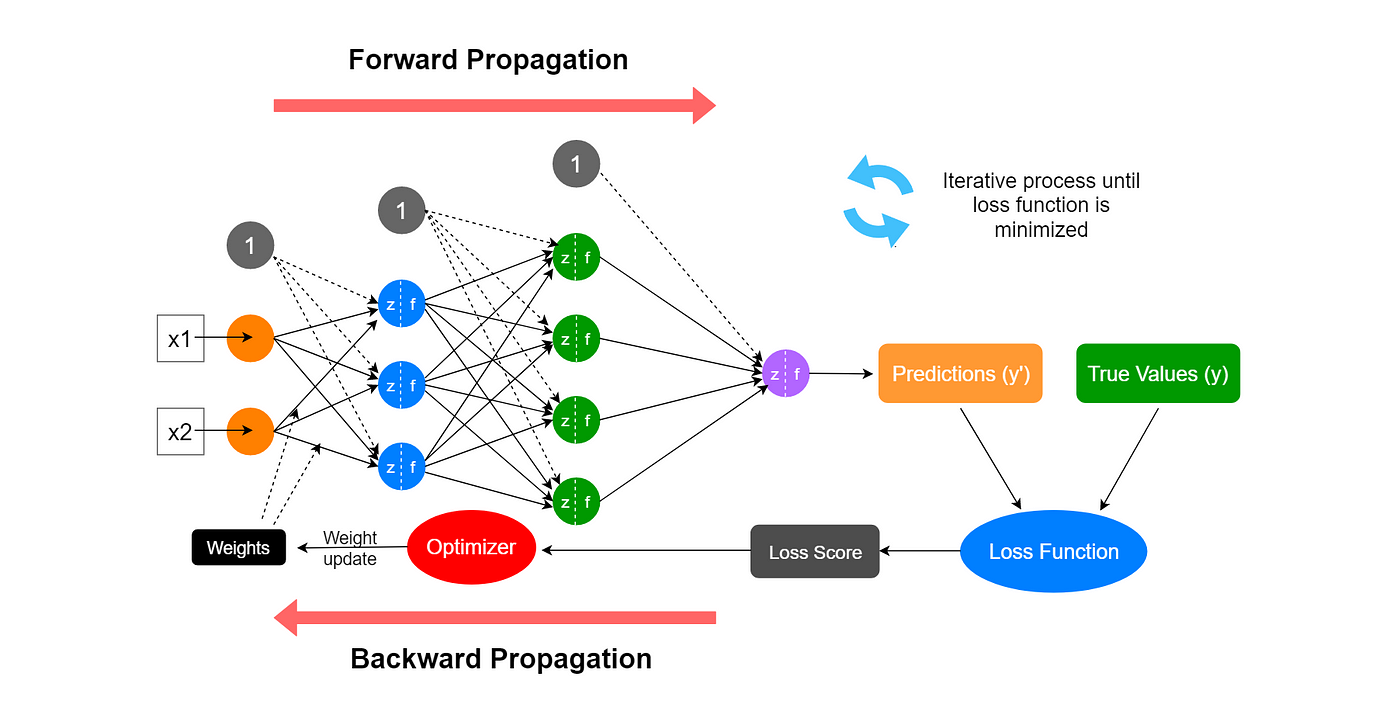
\includegraphics[width=\textwidth]{img/1_ZXAOUqmlyECgfVa81Sr6Ew.png}
    \captionof{figure}{Esempio di funzionamento di una rete neurale}
    \label{fig:NN_example}
\end{minipage}

Questo approccio tuttavia necessita di apprendere ogni aspetto della 
trasformazione non lineare direttamente dai dati a disposizione. In molti 
casi tuttavia, non è possibile conoscere l'intera equazione non lineare, 
ma magari se ne conosce la struttura generale. Il modo per definire 
matematicamente questo tipo di approccio è tramite le equazioni differenziali.
Il modo più immediato è quello di definire un modello matematico in 
cui si tenta di apprendere una costante associata all'andamento di un 
insieme di dati. 

$$y'(t) = \alpha \cdot y(t)$$

Tramite questo approccio non è necessario conoscere la soluzione dell'
equazione differenziale per convalidare che il modello sia corretto. Infatti 
la struttura del modellao e la matematica stessa viene codificata all'interno 
del modello stesso  il quale produce successivamente una soluzione. Questa 
tipologia di modelli è essenzialmente un insieme di equazioni che descrive 
il cambiamento delle cose e dove queste si troveranno ad un determinato periodo di tempo
è la soluzione al'equazione differenziale.

\begin{minipage}{\linewidth}
    \centering
    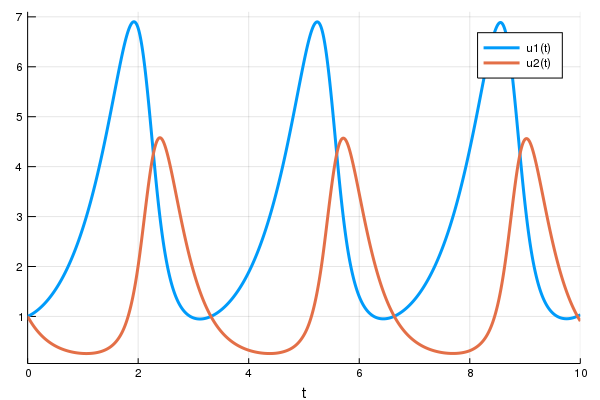
\includegraphics[width=\textwidth]{img/lotkavolterra.png}
    \captionof{figure}{Esempio grafico ODE rappresentante la famosa equazione di Lotka-Volterra}
    \label{fig:lotkavolterra_example}
\end{minipage}

Questo metodo è stata la soluzione utilizzata prevalentemente nel mondo 
della scienza e recentemente ha visto il proprio utilizzo ulteriormente 
espanso con l'ibridazione tramite strutture matematica aggiuntive che 
hanno permesso di modellare sistemi complessi come ad esempio la modellazione 
di sistemi farmacologici o biologici.

La peculiarità dei modelli di machine learning è che sono affamati di dati 
e richiedono un insieme di dati su cui allenarsi molto grande, e per questo 
l'utilizzo delle equazioni differenziali è divenuto un opzione molto 
interessante per specificare la nonlinearità in maniera apprendibile
(tramite parametri) in maniera limitata. Questo permette principalmente di 
incorporare una conoscenza specifica di un dominio nelle relazioni strutturali 
tra input e output del modello. 

Una equazione differenziale neurale è uno dei metodi per mettere in relazione
questi due mondi: quello del machine learning e quello delle equazioni differenziali.
L'approccio generale è quello di apprendere non tanto la trasformazione
non lineare che vi è tra i dati, quanto la struttura della trasformazione non 
lineare. Perciò invece che avere il modello $y = ML(x)$ avremo il modello 
$y' = ML(x)$ e si tenta successivamente di risolvere l'equazione differenziale 
associata.

Principalmente il motivo per cui si vuole utilizzare questa tipologia di approccio 
è quella per cui, definendo un modello in questo modo e utilizzando un risolutore
estremamente semplice e prono ad errori come il metodo di Eulero 
si ottengono risultati equivalenti ad una ResNet \cite{he2015deep}. L'idea alla base
è quella che invece di modellare una rete neurale con sempre più strati, e quindi 
sempre più profonda, è sufficiente modellare il sistema di equazioni differenziali
direttamente e successivamente risolverla tramite un risolutore specifico.

Questo tipo di approccio è \emph{memory efficient}, ha la capacità di gestire
\emph{dati irregolari} con forti priori sullo spazio del modello, ha un elevata
capacità di approssimare funzioni lineari e non lineari e si poggia su solide basi 
teoriche che pesca da entrambi i lati.

\subsubsection*{Risolvere una ODE in Julia}
L'idea alla base è quella di definire un oggetto \textbf{ODEProblem} tramite la 
definizione di una funzione che ha al suo interno la descrizione del sistema di ODE 
tramite la specificazione delle derivate delle equazioni nella forma $ù = f(u, p, t)$,
provvedendo a fornire un insieme di condizioni iniziali $u0$, un periodo di tempo $t$
e un insieme di parametri $p$.

\begin{minipage}{\linewidth}
    \centering
    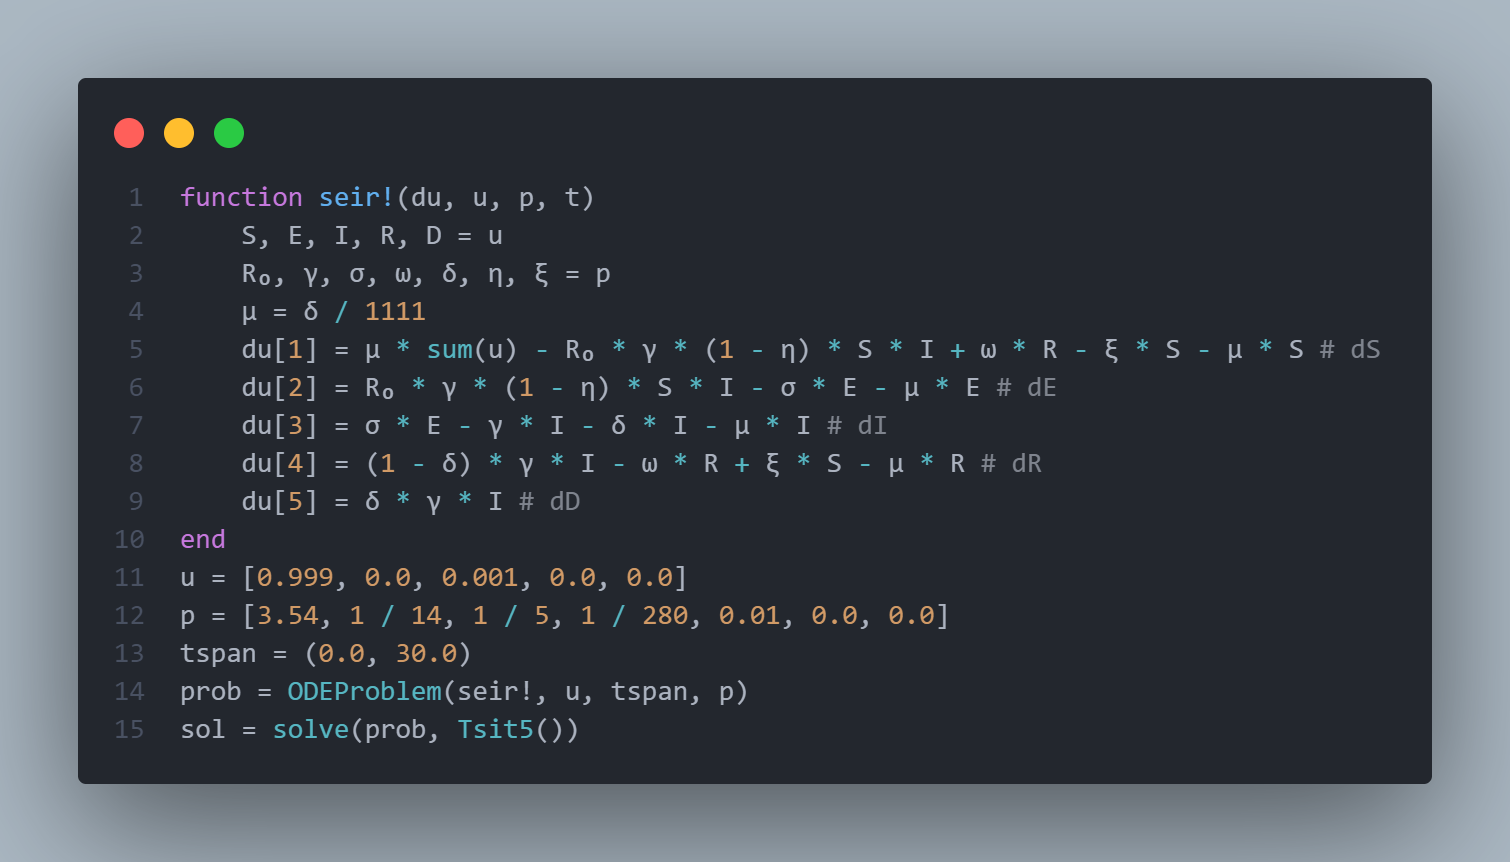
\includegraphics[width=\textwidth]{img/fdefinition.png}
    \captionof{figure}{Esempio definizione ODE in Julia}
    \label{fig:ODE_Julia_example}
\end{minipage}

Successivamente è possibile risolvere il sistema di ODE tramite la chiamata
della funzione \textbf{solve}

Si possono specificare molteplici metodi per la risoluzione del sistema, in 
questo caso il metodo \textbf{Tsit5} \cite{10.1016/j.camwa.2011.06.002} è un metodo 
di quinto ordine esplicito di tipologia \textbf{Runge-Kutta} con uno stimatore di errore
integrato di tipo \textbf{Tsitouras}. L'interfaccia proposta dal framework DifferentialEquations.jl 
permette di definire molteplici parametri aggiuntivi, utili per un approccio più capillare.

\subsubsection*{Inserire una ODE all'interno di una NN}
Per comprendere migliormente cosa significa inserire una ODE all'interno di una 
NN, bisogna osservare come un layer di una NN è definito. Un layer è sostanzialmente
una \emph{funzione differenziabile} che prende come input un vettore di dimensione $n$ 
e resituisce un nuovo vettore di dimensione $m$. Appare come i risolutori di DE rientrano 
anche loro nella categoria di funzioni differenziabili, il che significa che è possibile
inserirli direttamente all'interno di un programma differenziabile più grande.
Questo programma può essere nel nostro caso una rete neurale. 

\begin{minipage}{\linewidth}
    \centering
    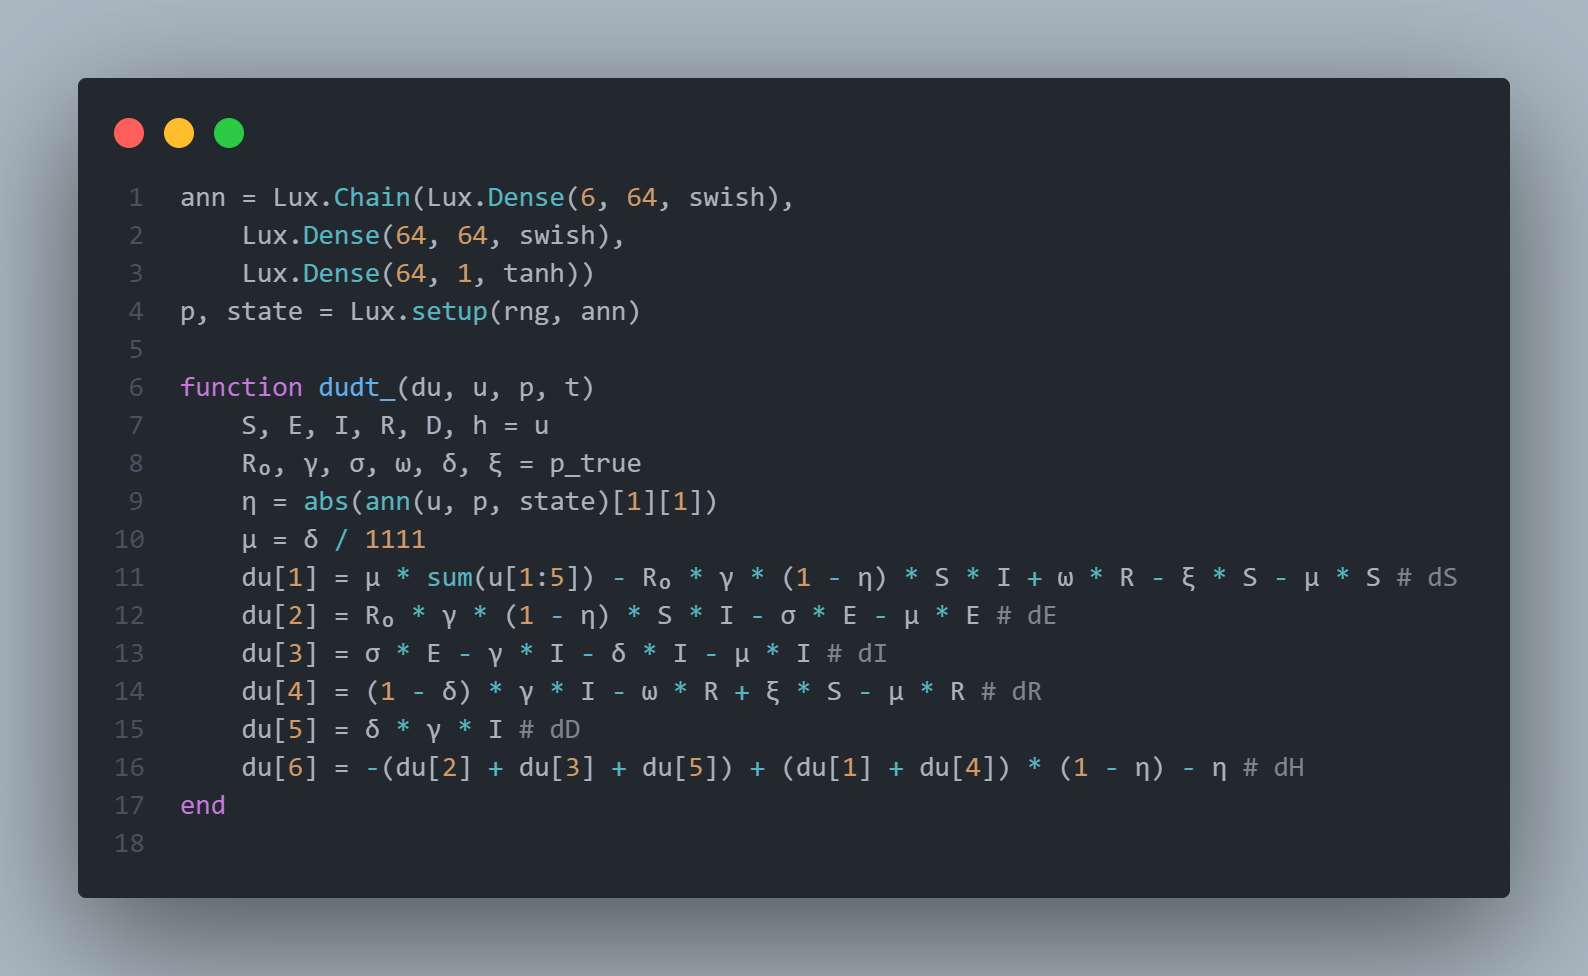
\includegraphics[width=\textwidth]{img/fann.png}
    \captionof{figure}{Esempio implementazione di una rete neurale in Julia}
    \label{fig:NN_Julia_example}
\end{minipage}

Successivamente è possibile addestrare per un determinato numero di integrazioni 
la nostra rete neurale per ottenerne i risultati. 

è importante puntualizzare come il sistema non stia apprendendo una soluzione all'
equazione differenziale. Piuttosto ciò che sta imparando è il sistema di ODE da cui 
la soluzione è generata. In questo caso la Neural ODE impara una rappresentazione 
compatta di come la serie di dati si comporta nel tempo, e può facilmente estrapolare
cosa potrebbe succedere con differenti condizioni iniziali. La suite \textbf{DiffEqFlux.jl} \cite{chen2019neural} permette di avere un comodo wrapper 
per definire una \textbf{NeuralODE}.

\begin{minipage}{\linewidth}
    \centering
    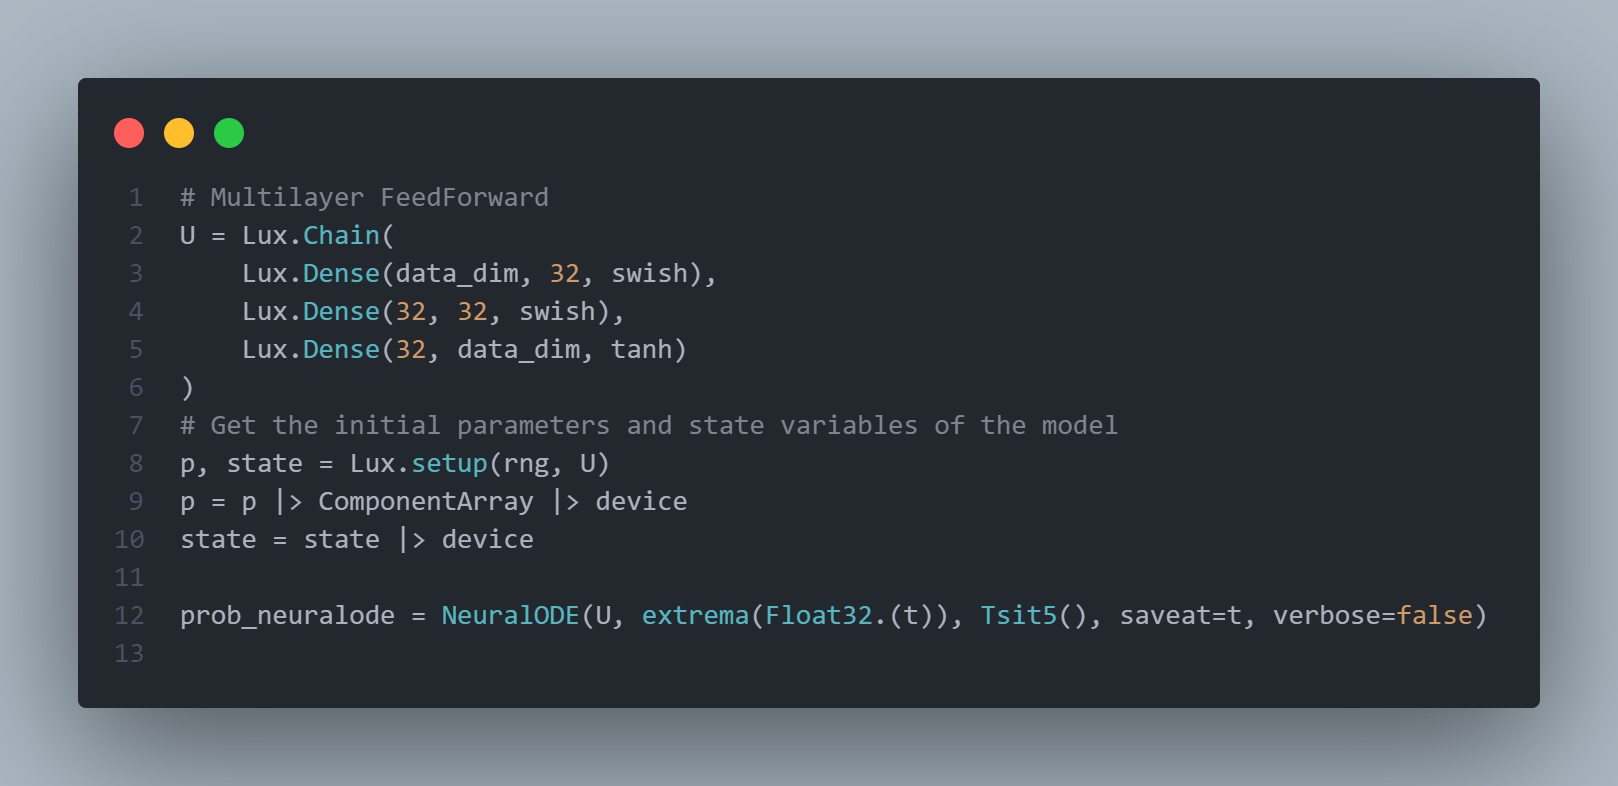
\includegraphics[width=0.8\textwidth]{img/fneuralode.png}
    \captionof{figure}{Esempio implementazione NeuralODE tramite DiffEqFlux.jl}
    \label{fig:NeuralODE_Julia_example}
\end{minipage}

\subsubsection*{Backpropagation tramite ODE solver}
Il cuore di ogni rete neurale è l'abilità di propagare all'indietro lungo tutta la 
rete le derivate, con lo scopo di calcolare il gradiente della funzione di perdita
rispetto ai parametri della rete. Perciò la sfida diventa trovare un metodo per
applicare lo stesso comportamento anche quando si utilizzano dei risolutori ODE 
all'interno della rete neurale.

Esistono svariati approcci, il più comune è tramite un approccio di analisi di sensitività (adjointed).
L'analisi di sensitività definisce una nuova ODE la cui soluzione fornisce il gradiente per 
la funzione di costo rispetto ai parametri, e successivamente viene risolta questa seconda
ODE.

\subsubsection*{Equazioni Ordinarie Differenziali}
Nell'ambito matematico, una \emph{equazione ordinaria differenziale} (ODE) è un 
equazione differenziale (DE) dipendente da un singolo valore indipendente, 
generalmente il tempo. All'interno di questa grande famiglia di equazioni, 
il gruppo delle \emph{equazioni lineari differenziali} gioca un ruolo predominante
in quanto la maggior parte dei fenomeni fisici e di matematica applicata possono 
essere descritti dalla soluzione di questo tipo di equazioni. 

Una equazione lineare differenziale è definita da un \emph{polinomio lineare} 
e la sua derivata è un equazione dalla forma:

$$\alpha_0(x)y + \alpha_1(x)y' + \alpha_2(x)y'' + ... + \alpha_n(x)y^{(n)} + b(x) = 0$$

dove $\alpha_0(x), ..., \alpha_n(x)$ e $b(x)$ sono funzioni differenziabili arbitrarie che non 
richiedono di essere lineari, e $y', ..., y^{(n)}$ sono le successive derivate della funzione incognita
$y$ della variabile $x$.

L'utilizzo di \emph{equazioni non lineari differenziali} può essere 
generalmente approssimato con la controparte lineare così da ottenere una 
soluzione più semplice. 

La suite di SciML.ai offre un ampia varietà di framework per la risoluzione di sistemi di 
equazioni lineari differenziali i quali si possono prevalentemente trovare 
all'interno della libreria \emph{DifferentialEquations.jl} \cite{rackauckas2017differentialequations}
\cite{rackauckas2019confederated} \cite{9622796} \cite{gowda2019sparsity},
i risolutori sono molteplici e permettono grande dinamicità e affidabilità 
nonchè elevate prestazioni durante l'utilizzo, questo in relazione anche ai risolutori dei più 
conosciuti linguaggi di programmazione come ad esempio: \textbf{MATLAB, SciPy, R, C e C++ e altri}.

La figura riportata sotto \ref{fig:de_comparison_table} \cite{10.15200/winn.153459.98975} mostra una comparativa tra le varie implementazioni dei 
metodi di risoluzione di sistemi di ODE di vario genere utilizzati dalla maggior
parte dei linguaggi di programmazione focalizzati sull'analisi numerica e scientifica.

\begin{minipage}{\linewidth}
    \centering
    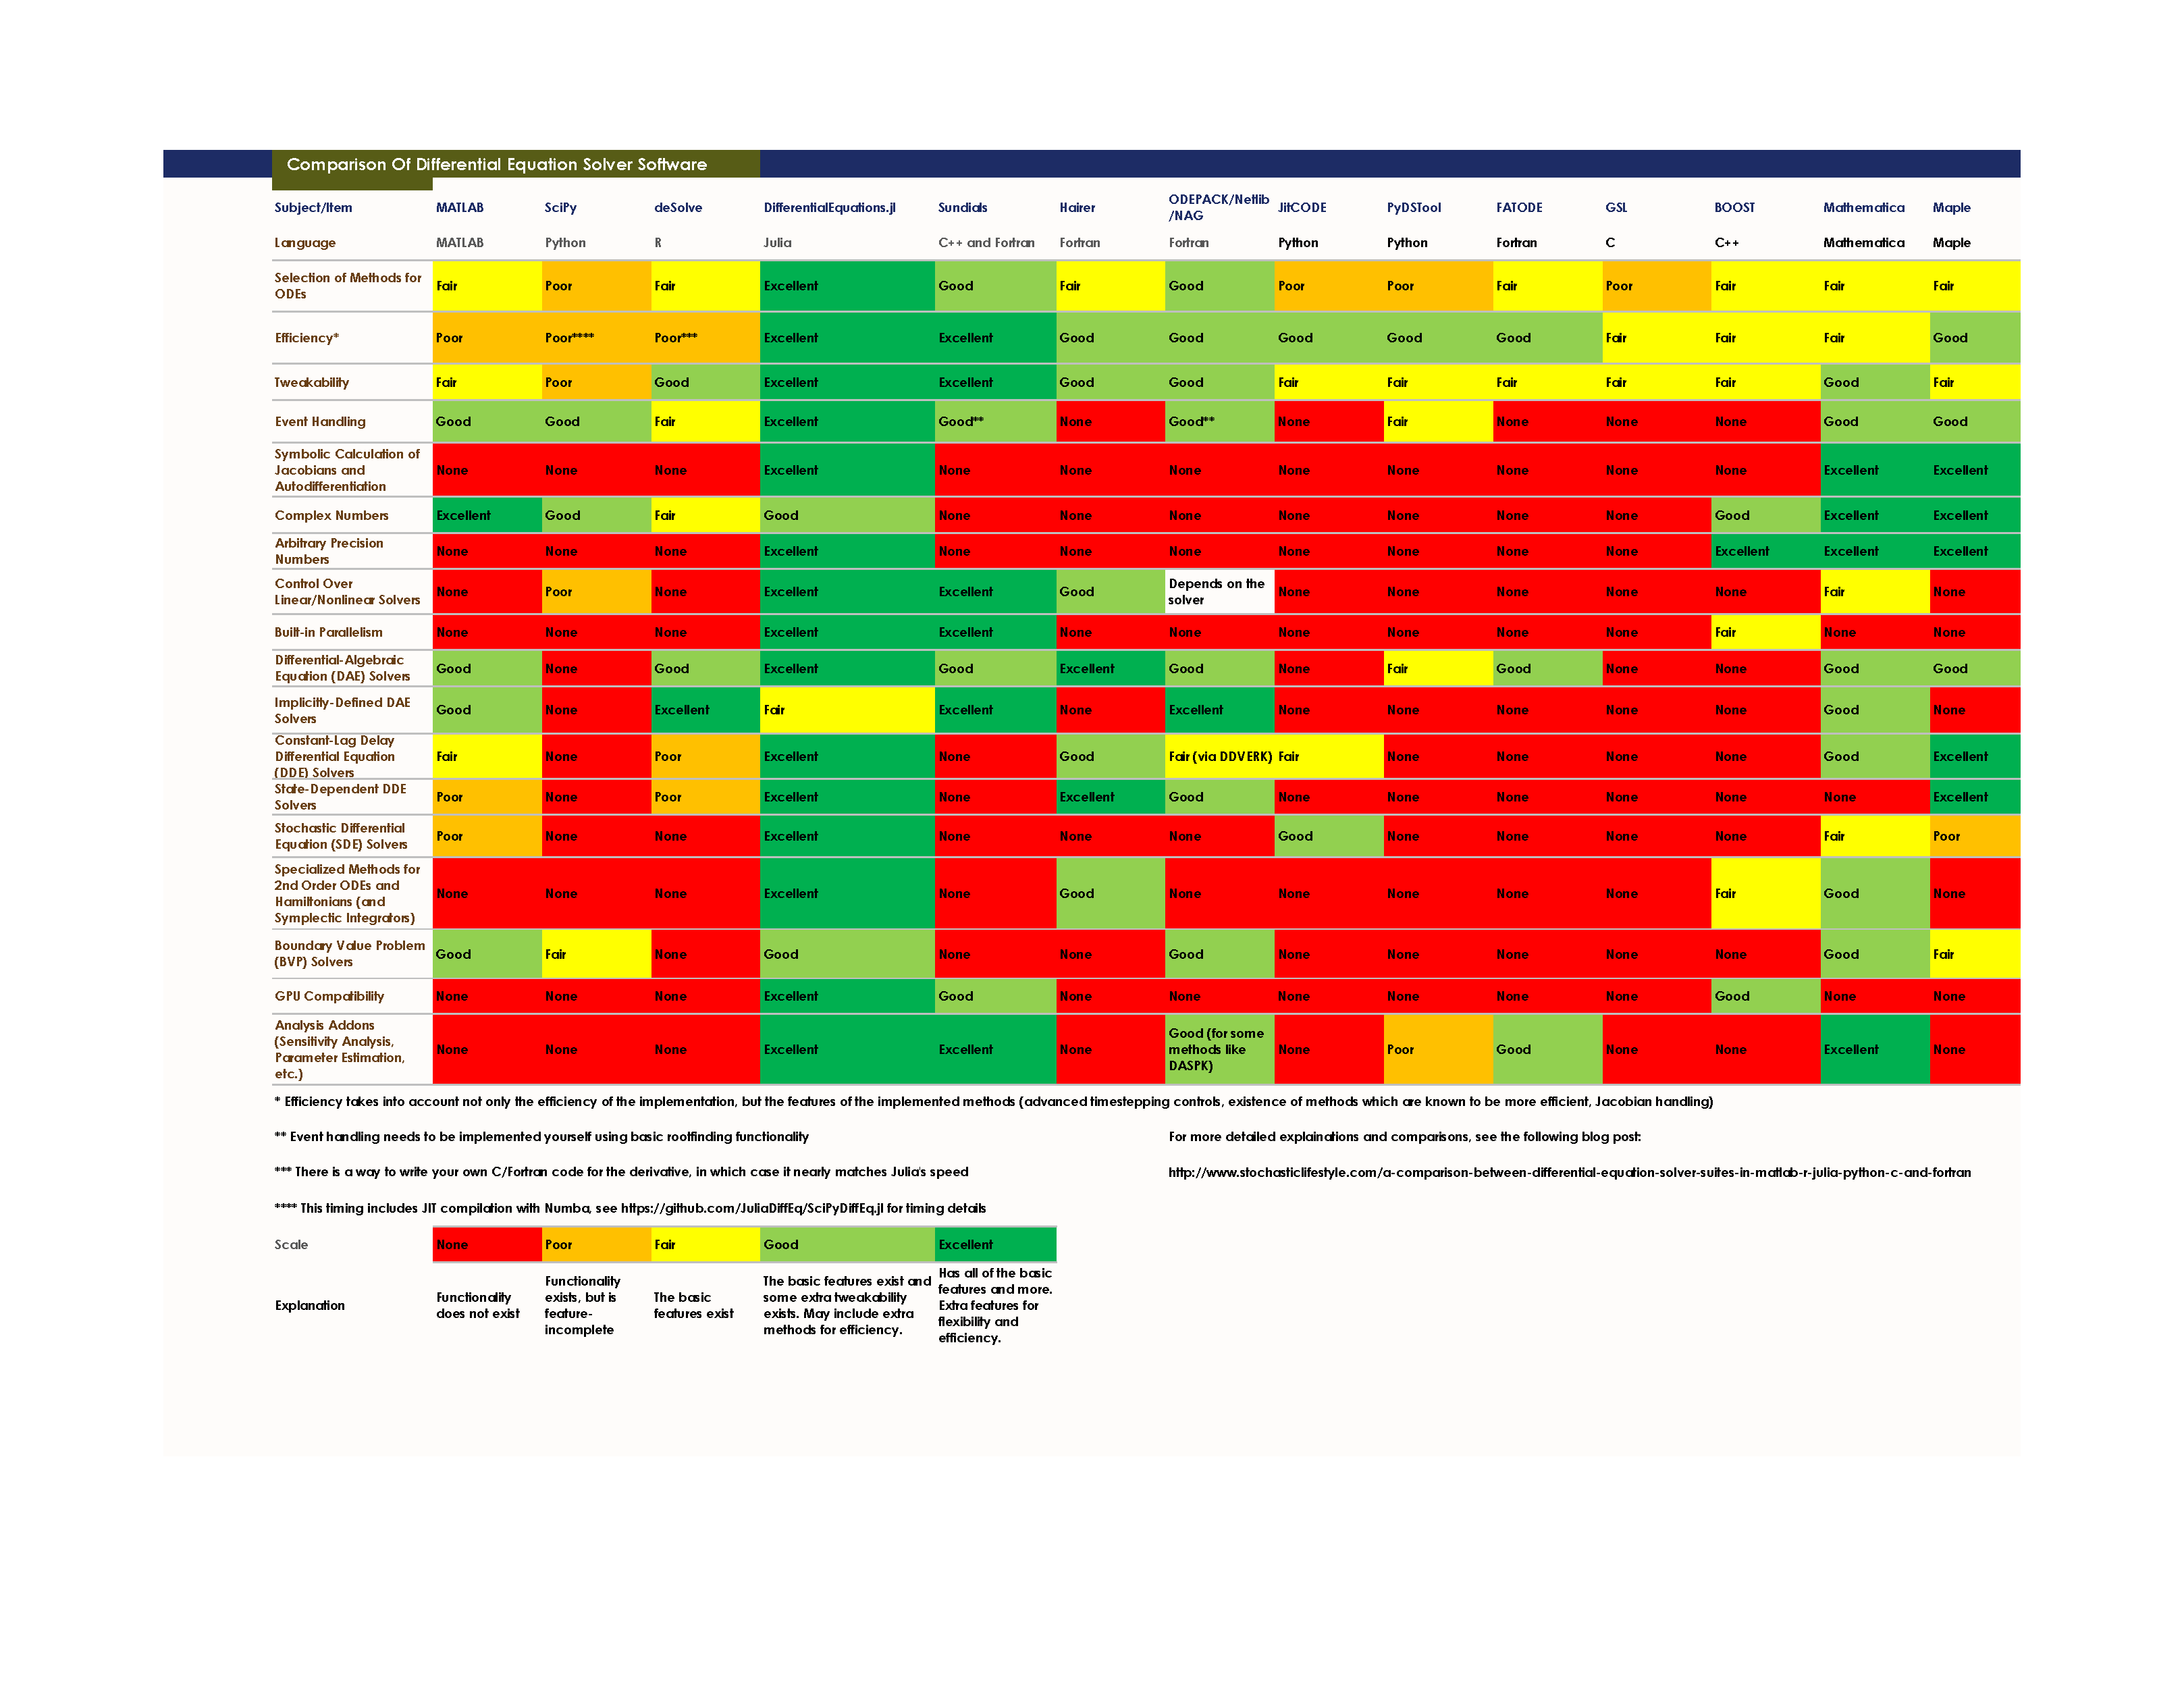
\includegraphics[width=\textwidth]{img/de_solver_software_comparsion.pdf}
    \captionof{figure}{Tabella comparativa tra le varie implementazioni dei vari risolutori \cite{10.15200/winn.153459.98975}}
    \label{fig:de_comparison_table}
\end{minipage}

\subsubsection*{Equazioni Differenziali Universali}
Recentemente gli avanzamenti nel mondo del machine learning sono stati dominati dalle tecniche 
di deep learning le quali necessitano di una quantità di dati enormi, generalmente chiamati \emph{big data}, 
per risolvere problemi definiti precedentemente come difficili e complessi, come ad esempio problemi di 
\emph{image recognition} o \emph{natural language processing}. 

\begin{minipage}{\linewidth}
    \centering
    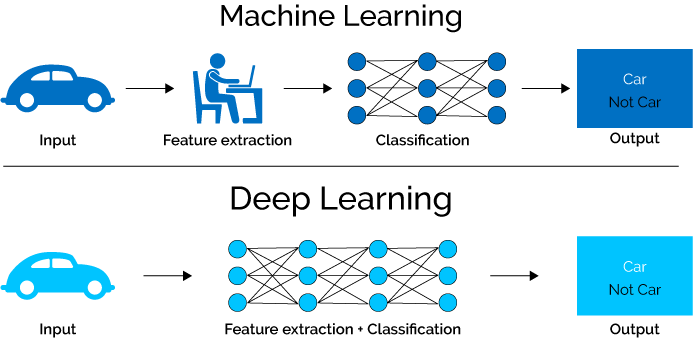
\includegraphics[width=\textwidth]{img/Caratteristiche-e-funzionamento-del-Deep-Learning-in-informatica.png}
    \captionof{figure}{Esempio comparativo tra funzionamento Machine Learning e Deep Learning}
    \label{fig:ml_dl_example}
\end{minipage}

Tuttavia se molteplici ambiti della scienza sono riusciti a generare una mole di dati sufficiente per l'utilizzo di 
queste tecniche, alcuni ambiti specialmente legati alla medicina e a tutto ciò che ne concerne, faticano enormemente
ad avere un insieme di dati sufficientemente grande e variegato per applicare le tecniche sopra introdotte. In questo 
ambito i modelli meccanicistici rimangono quelli più utilizzati. L'utilizzo di questi modelli tuttavia impone dei limiti 
quali l'essere modelli predittivi che dipendono fortemente dalle conoscenze pregresse del modello, andando a creare quello 
che può essere assimilabile ad una specie di bias induttivo, mentre l'approccio data-driven dei modelli di machine learning 
può consentire di essere molto più flessibile permettendo di abbandonare le ipotesi semplificative 
necessarie per derivare i modelli teorici. 

Un \emph{equazione differenziale universale} (UDE) è un insieme di equazioni differenziali definiti pienamente,
o in parte, da un \emph{approssimatore universale}. Un approssimatore universale è un oggetto parametrico 
capace di rappresentare qualsiasi funzione dato una determinata dimensione dei parametri. Degli approssimatori 
universali, in uno spazio a basse dimensioni includono la serie di Fourier o di Chebyshev, mentre un 
approssimatore universale in uno spazio ad alte dimensioni includono le reti neurali e altri modelli utilizzati 
all'interno del machine learning. Matematicamente parlando però, nella sua forma più generale, una UDE è 
una equazione differenziale parziale (PDE) a ritardo stocastico forzato definita con approssimatori universali incorporati:
$$\mathcal{N}[u(t), u(\alpha(t)), W(t), U_\theta(u, \beta(t))] = 0$$
dove $\alpha(t)$ è una funzione a ritardo e $W(t)$ è un processo Wiener.

Un \emph{equazione differenziale universale} (UDE) è una \emph{equazione algebrica
differenziale} 
non triviale, ovvero un sistema di equazioni che contiene delle equazioni differenziali
ed equazioni algebriche oppure è un sistema equivalente,
con la proprietà che la sua soluzione può approssimare
\emph{qualsiasi} funzione continua su un qualunque intervallo $\in R$ a 
qualsiasi livello di precisione desiderata. 

Per essere precisi, una equazione differenziale (possibilmente in forma implicita)
$P( y', y'', y''', ..., y^{(n)})=0$ è una UDE se, per ogni funzione a valori relative
continua $f$ e per ogni funzione continua positiva $\epsilon$ esiste una 
soluzione liscia (una funzione è considerabile liscia se è 
differenziabile in ogni suo punto, perciò continua) $y$ di $P( y', y'', y''', ..., y^{(n)})=0$
con $|y(x) - f(x)| < \epsilon(x) \forall x \in R$.

Il concetto di UDE può essere analogo all'idea di una \emph{Macchina di Turing Universale}
con la differenza che le UDE non dettano 
l'evoluzione di un sistema, ma si limitano a imporre determinate regole che 
ogni sistema che si evolve deve sodddisfare. Questo permette di avere un modello robusto 
per l'analisi di dati e la predizione dell'interazione che hanno vari fenomeni tra loro.

\begin{minipage}{\linewidth}
    \centering
    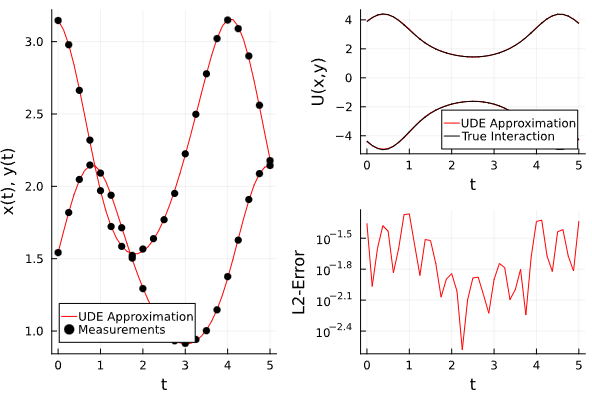
\includegraphics[scale=0.7]{img/ude_approx.png}
    \captionof{figure}{Comportamento UDE nell'approssimazione di fenomeni non lineari}
    \label{fig:UDE_approx}
\end{minipage}

Questo approccio viene spesso unito a tecniche \emph{Data-Driven} \cite{datadrivendiffeq} per l'identificazione
sparsa di dinamiche non lineari. In particolare uno degli approcci utilizzati 
è quello tramite l'algoritmo \emph{SINDy (\textbf{S}parse \textbf{I}dentification of \textbf{N}on-linear \textbf{Dy}namics)}. 
Questo algoritmo performa una serie di operazioni di regressione come 
ad esempio \textbf{LASSO} su una libreria di funzioni candidate non lineari ottenute
da uno snapshot del sistema dinamico che si sta analizzando e delle sue derivate, 
con l'obiettivo di trovare le equazioni che lo governano. Questo procedimento 
si basa sull'assunzione che molti sistemi fisici hanno solamente una manciata di 
termini che ne dettano le dinamiche e l'evoluzione. Questo metodo è stato largamente
utilizzato nell'identificazione della \emph{dinamica dei fluidi} così come
nelle \emph{reti biologiche} e altri sistemi dinamici complessi.